\documentclass{article}

\usepackage{graphicx}
\usepackage{hyperref}
\usepackage{cleveref}
\usepackage{subcaption}

\title{Hermes: Final Report}

\title{Hermes: Final Report}
\author{Clark Barrett, Mathias Preiner, Yoni Zohar
\date{Stanford University}}
\begin{document}
\maketitle

\section{Query Dispatcher}
\subsection{Description}
Part of the approach that underlies the HERMES project is
``choosing the right tool for the job``.
And indeed, sub-problems that are described in
a HERMES module are dispatched to various
reasoning engines such as SMT-solvers, model checkers, etc.
This approach can be leverged also in a lower level of abstraction.
When a (sub-)problem that is decided by HERMES to be solved by an SMT-solver, it is still
required to determine \emph{which} SMT-solver will be used.

For this purpose, we have implemented and utilized a
{\em query dispatcher}, that
makes use of the fact that several solvers
can be run in parallel.
Thus, given an input file written in the SMT-LIB standard \cite{SMTLib2010}, we dispatch it to several solvers in parallel,
return the result obtained by the first solver to get an answer, and
terminate the runs of the rest of the solvers.

In order to not overuse system resources, and given the large number of SMT-solvers,
not all possible solvers are executed, but a subset of them is being chosen.
To choose this subset efficiently, we need to decide which subset of solvers is best
for the input problem.
The parameter of the input problems that we chose to focus on is the problem's {\em logic}.
Problems in SMT-LIB format are divided into logics, that determine the various types and operators
that are allowed to be used.
Prominent such logics include, e.g.,
QF\_BV, the quantifier-free logic of bit-vectors,
QF\_NRA, the quantifier-free logic of non-linear real arithmetic,
UFNIA, the quantified logic of non-linear integer arithmetic combined with uninterpreted functions, etc.

Given the input problem's logic (which is typically specified in the first line of
the input SMT-LIB file), we employ a data-driven approach to project which solvers should be used.
For each logic, we choose the solvers that were in the first four places in
the yearly SMT competition \cite{DBLP:journals/jsat/WeberCDHNR19}.
The current version of the dispatcher relies on the results from the 2019 competition \cite{smtcomp2019}.
In case less than four solvers are supported for the given logic, all of them are chosen.

The dispatcher currently supports the following pool of solvers:
CVC4 \cite{CVC4},
Z3 \cite{Z3},
Yices \cite{Dutertre:cav2014},
VERIT \cite{10.1007/978-3-642-02959-2_12},
mathsat \cite{mathsat5},
and
SPASS\_SATT \cite{10.1007/978-3-030-29436-6_7}.


In addition to the above functionallity, the dispatcher allows the user to manually choose
which solvers will be used, by specifying a list of their names in the command line.

The following snippet is a trace from running the dispatcher.
In each line, there is a timeout of 3 seconds which is enforced on the command that
is being executed (using \verb!timeout 3s!).
In the first line, CVC4 is specified by the user as the chosen solver, 
and returns a result.
Next, Yices is chosen to run on the same file, and does not return a result.
In the next two commands, a different benchmark is used with the opposite results:
Yices returns an answer while CVC4 does not.
Next, the \verb!-s! option of the tool allows the user to specify more than one solver,
and so when both CVC4 and Yices are specified, a result is obtained.
Finally, the \verb!normal! keyword of the tool invokes the selection algorithm
described above, which succesfully results in a solution.

\begin{center}
\begin{verbatim}
$ timeout 3s python3 dispatcher.py term-mzEEAc.smt2 -s cvc4
sat
$ timeout 3s python3 dispatcher.py term-mzEEAc.smt2 -s yices
$ timeout 3s python3 dispatcher.py term-n2YjEt.smt2 -s cvc4
$ timeout 3s python3 dispatcher.py term-n2YjEt.smt2 -s yices
sat
$ timeout 3s python3 dispatcher.py term-n2YjEt.smt2 -s cvc4 yices
sat
$ timeout 3s python3 dispatcher.py term-n2YjEt.smt2 -s normal
sat
\end{verbatim}
\end{center}

\subsection{Evaluation}

Since the dispatcher chooses the best performing solvers based on
the SMT-LIB competition
and runs them in parallel,
it is expected that it will outperform any single solver,
unless it introduces overhead that skews these results.
Luckily, the dispatcher is lightweight and performs
as expected.

To show this, we compared the performance of the dispatcher
with the performance of two mainstream SMT-solvers,
namely Z3 and CVC4.
As a benchmark set for the experiments we used the benchmarks that were chosen for the 2019 SMT competition in the single-query track on two divisions:
QF\_NRA and QF\_NIA.
These divisions include non-linear arithmetic formulas
over the reals and integers, respectively.
We measured how many benchmarks were solved as time
elapsed, with
a time limit of 5 minutes and memory limit of 8GB.
%
The experiments were done on
a cluster with Intel Xeon CPUE5-2620 CPUs with 2.1GHz and 128GB memory.
The results of this evaluation are presented in
\Cref{cactus,scatternra,scatternia}.

\Cref{cactus} contains two cactus plots.
In each plot, each point corresponds to a benchmark, and it
is placed on the y-axis according to the time
it took to solve the benchmark (or to reach a timeout).
The points are ordered according to their corresponding
running times on the different solvers, and so
two points at the same position according to the x-axis
do not necessarily describe the same benchmark.
The left plot describes the results on QF\_NRA and
the right one describes the results on QF\_NIA.
Consistently, the dispatcher solved more benchmarks
than Z3 and CVC4, overall and also at every time period,
for both logics.

\Cref{scatternra} contains two scatter plots.
In these plots, every point corresponds to a benchmark
from the QF\_NRA family,
and it is placed on the x-axis according to the
solving time using CVC4 (on the left) and Z3 (on the right),
and on the y-axis according to the solving time using
the dispatcher.
%
Thus, points that are on the main diagonal correspond to benchmarks that
were solved equally fast by the dispatcher and CVC4/Z3,
and points below the main diagonal correspond
to benchmarks on which the dispatcher performed
faster.
%
As noted in the plots' legends, the color of the points
describes by which factor was the better-performing solver faster.
%
It can be clearly seen that most of the points are below the main diagonal on both plots,
which means that the dispatcher performed better
than CVC4 and Z3 on QF\_NRA.
%
\Cref{scatternia} presents similar results for QF\_NIA formulas.

Overall, out of 2842 QF\_NRA benchmarks,
the dispatcher solved 2584 in the given time limit,
Z3 solved 2134, and
CVC4 solved 1542.
%
Out of 11494 QF\_NIA benchmarks,
the dispatcher solved 8637 in the given time limit,
Z3 solved 4782, and
CVC4 solved 6320.


\begin{figure}
\begin{center}
\begin{tabular}{cc}
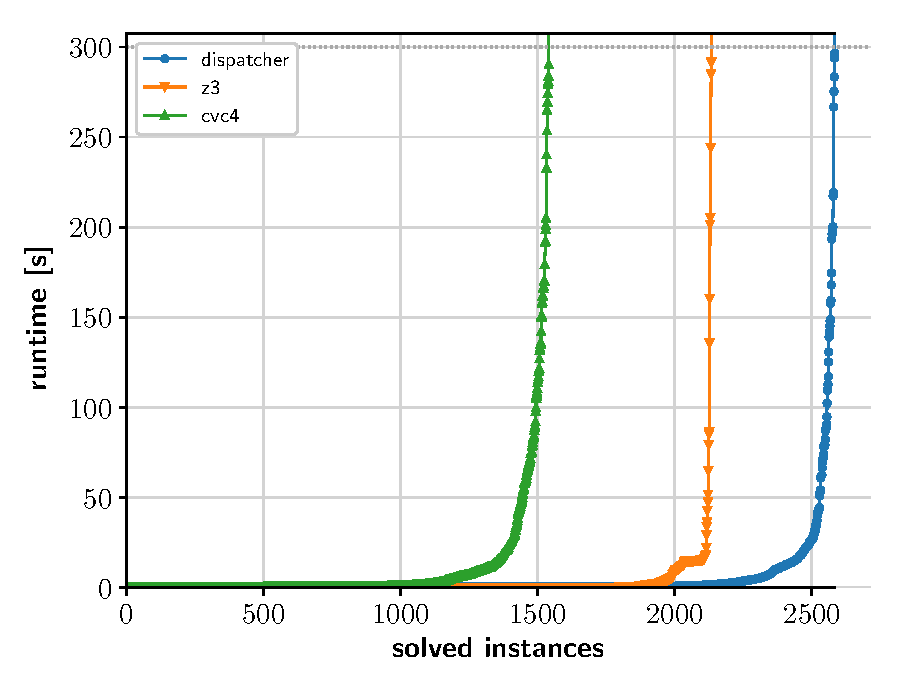
\includegraphics[width=.5\textwidth]{plot/cactus_qfnra_dispatcher_cvc4_z3}
&
\includegraphics[width=.5\textwidth]{plot/cactus_qfnia_dispatcher_cvc4_z3}  
\end{tabular}
\end{center}
\caption{\label{cactus}Cactus Plots comparing the dispatcher, Z3 and CVC4 on benchmarks from QF\_NRA and QF\_NIA.}
\end{figure}


\begin{figure}
\begin{center}
\begin{tabular}{cc}
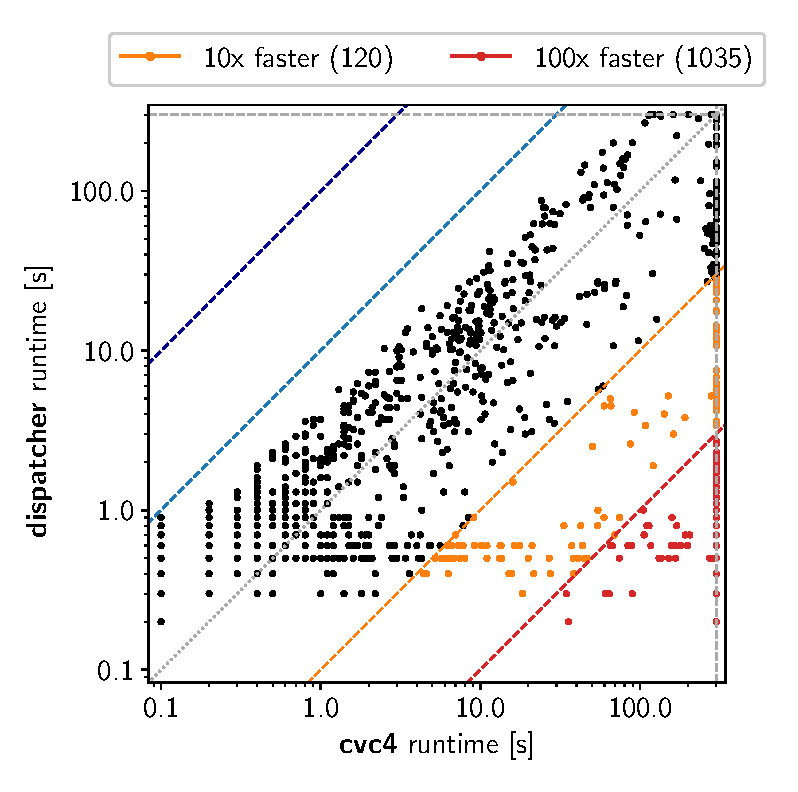
\includegraphics[width=.5\textwidth]{plot/scatter_qfnra_dispatcher_cvc4}
&
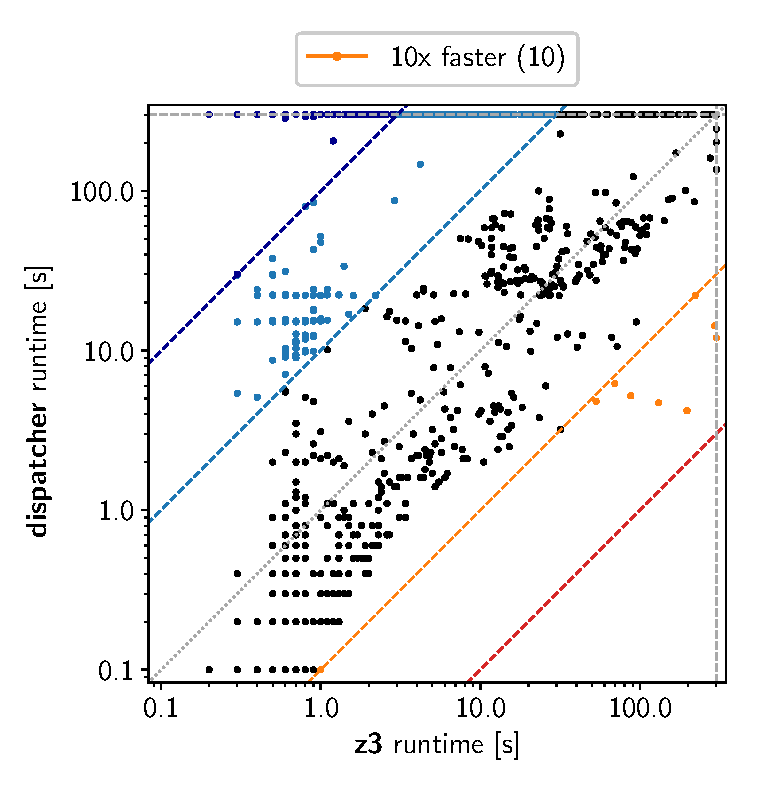
\includegraphics[width=.5\textwidth]{plot/scatter_qfnra_dispatcher_z3} 
\end{tabular}
\end{center}
\caption{\label{scatternra}Scatter plots comparing the dispatcher against Z3 and CVC4 on benchmarks from QF\_NRA.}
\end{figure}

\begin{figure}
\begin{center}
\begin{tabular}{cc}
\includegraphics[width=.5\textwidth]{plot/scatter_qfnia_dispatcher_cvc4}
&
\includegraphics[width=.5\textwidth]{plot/scatter_qfnia_dispatcher_z3}  
\end{tabular}
\end{center}
\caption{\label{scatternia}Scatter plots comparing the dispatcher against Z3 and CVC4 on benchmarks from QF\_NIA.}
\end{figure}



\section{Algorithm Selection for SMT}

Using a parallel portfolio of SMT solvers to solve a problem will give you
the best performance if the best solvers are run in parallel. However, the
solver selection is not very flexible,
and is (currently) limited to only taking the logic into account.
Also, the number of solvers to
be run in parallel is limited by available resources.

We investigated leveraging machine learning techniques to automate the
solver selection while also reducing the resources required to solve problems.
The general idea of this approach is to train a model that can predict which
solver will be the fastest to solve a given problem based on features extracted
from the problem.
In collaboration with Joseph Scott and Vijay Ganesh from the University of
Waterloo we developed such an algorithm selection tool called
MachSMT~\footnote{\url{https://github.com/j29scott/MachSMT}}.

\subsection{Overview}

MachSMT employs empirical hardness models (EHMs)~\cite{leyton2002learning}
to perform algorithm selection.
It uses the number of occurrences of grammatical constructs from the
SMT-LIB language as features in combination with principal component analysis
(PCA)~\cite{pca} and Adaptive Boosting (AdaBoost)~\cite{drucker1997improving}
to construct an EHM for each solver.
An EHM for a given solver $S$ is a mapping from an input instance $I$ to a
predicted runtime of $S$ on $I$.
During evaluation or at runtime, given an input instance $I$, MachSMT queries
all EHMs for all solvers (that were considered during training) over $I$, and
outputs the solver name whose predicted runtime is the minimum over all
solvers.

\subsection{MachSMT Workflow}

Figure~\ref{fig:machsmt} shows the overall workflow of MachSMT.
To build models, MachSMT expects runtime data for a set of solvers on a set of
input problems by means of a CSV file with columns \texttt{benchmark},
\texttt{solver}, \texttt{score}.
The \texttt{score} can be any value that the users wants to optimize for.
In our case, it is the time required to solve a benchmark.
Optionally, the user can provide custom features that will be considered when
constructing EHMs.
As a first step, MachSMT extracts features from each benchmark that are not yet
in the feature database.
It then constructs an EHM for each solver on the benchmarks in the given
dataset.
Once all EHMs are constructed the user can query MachSMT (selector) with a new
input problem for which MachSMT will predict the fastest solver, which can then
be used by the user to solve the input problem.

Note that it is not required to rebuild the EHMs each time, but only if the
training data set changes, e.g., when a user wants to include additional
solvers or wants to train on a different family of input problems.

\begin{figure}
  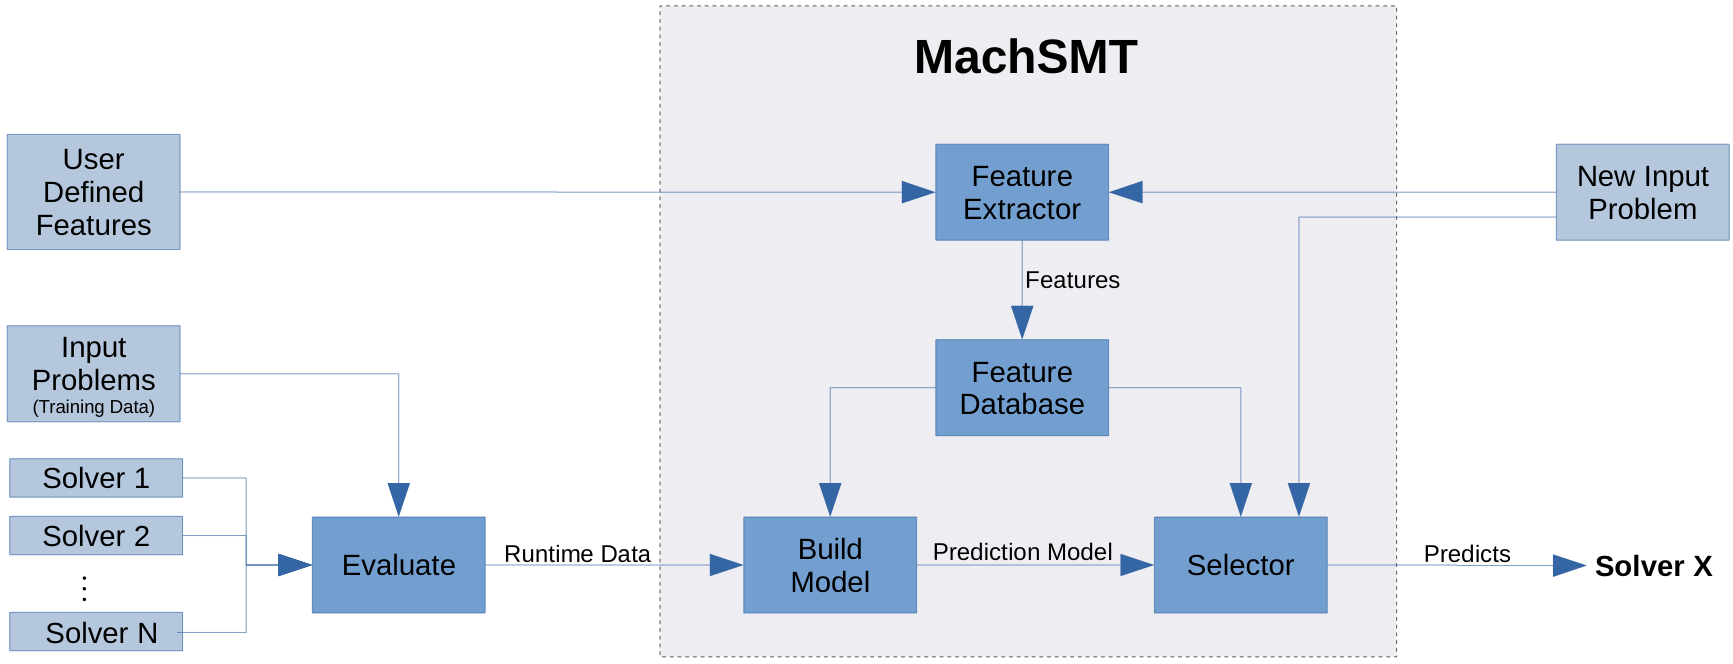
\includegraphics[width=\textwidth]{machsmt.png}
  \caption{MachSMT workflow.}
  \label{fig:machsmt}
\end{figure}

\subsubsection{Features and Preprocessing}

MachSMT uses a feature vector with 148 entries, where each entry corresponds to
a grammatical construct in the SMT-LIB language, e.g., commands like
\texttt{assert}, \texttt{declare-const}, or
theory symbols like \texttt{bvmul}, \texttt{fp.add}.
Given an input instance, a script first computes the number of occurrences for
each grammatical construct and populates the corresponding feature vector
appropriately.
MachSMT then performs the following preprocessing steps before constructing any
learned models over a given dataset.
First, all feature values are scaled to zero mean and unit variance, then
polynomial features of degree two is computed, which is a common normalization
in machine learning research.
To prevent potential issues caused by a high dimensional feature space, we then
apply principal component analysis and use the first 35 components, which
results in a smaller feature vector and prevents further feature selection.
The number of selected components was determined empirically.


\subsubsection{User-defined Features}

MachSMT provides a simple interface that allows users to define custom features
by means of implementing a function in Python that returns a single
floating-point number that represents a feature.
The input to the function is the path to the input problem.
If a user feature is to be considered by MachSMT, the user-defined function
should return its floating-point representation, otherwise returns
\texttt{None}.
All user-defined features will be automatically included while building models
with MachSMT.


\subsection{Evaluation}

We evaluated MachSMT on runtime data provided by the annual SMT competition
from 2019 (SMT-COMP 2019) \cite{smtcomp2019}.

In order to avoid overfitting in our evaluation, we perform $k$-fold cross
validation (with $k = 5$) to randomly partition the dataset into $k$ subsets.
A model is then trained over $k - 1$ subsets and asked to make predictions over
the subset that is excluded from training.
This process is repeated $k$ times per EHM in order to obtain a fair prediction
for each input problem.

We trained MachSMT on the SMT-COMP 2019 data on each division and compared
it against all solvers participating in this division.
We also compare MachSMT against the virtual best solver, which essentially
corresponds to the dispatcher running all SMT solvers of the division in
parallel.

Figure~\ref{fig:machsmt_results} shows the results on selected SMT-COMP
divisions in terms of cactus plots.
In each of these divisions, MachSMT was able to beat the winner of the division
and further was able to get very close to the virtual best solver in the
QF\_UFBV division.

\begin{figure}
  \begin{subfigure}{0.48\textwidth}
    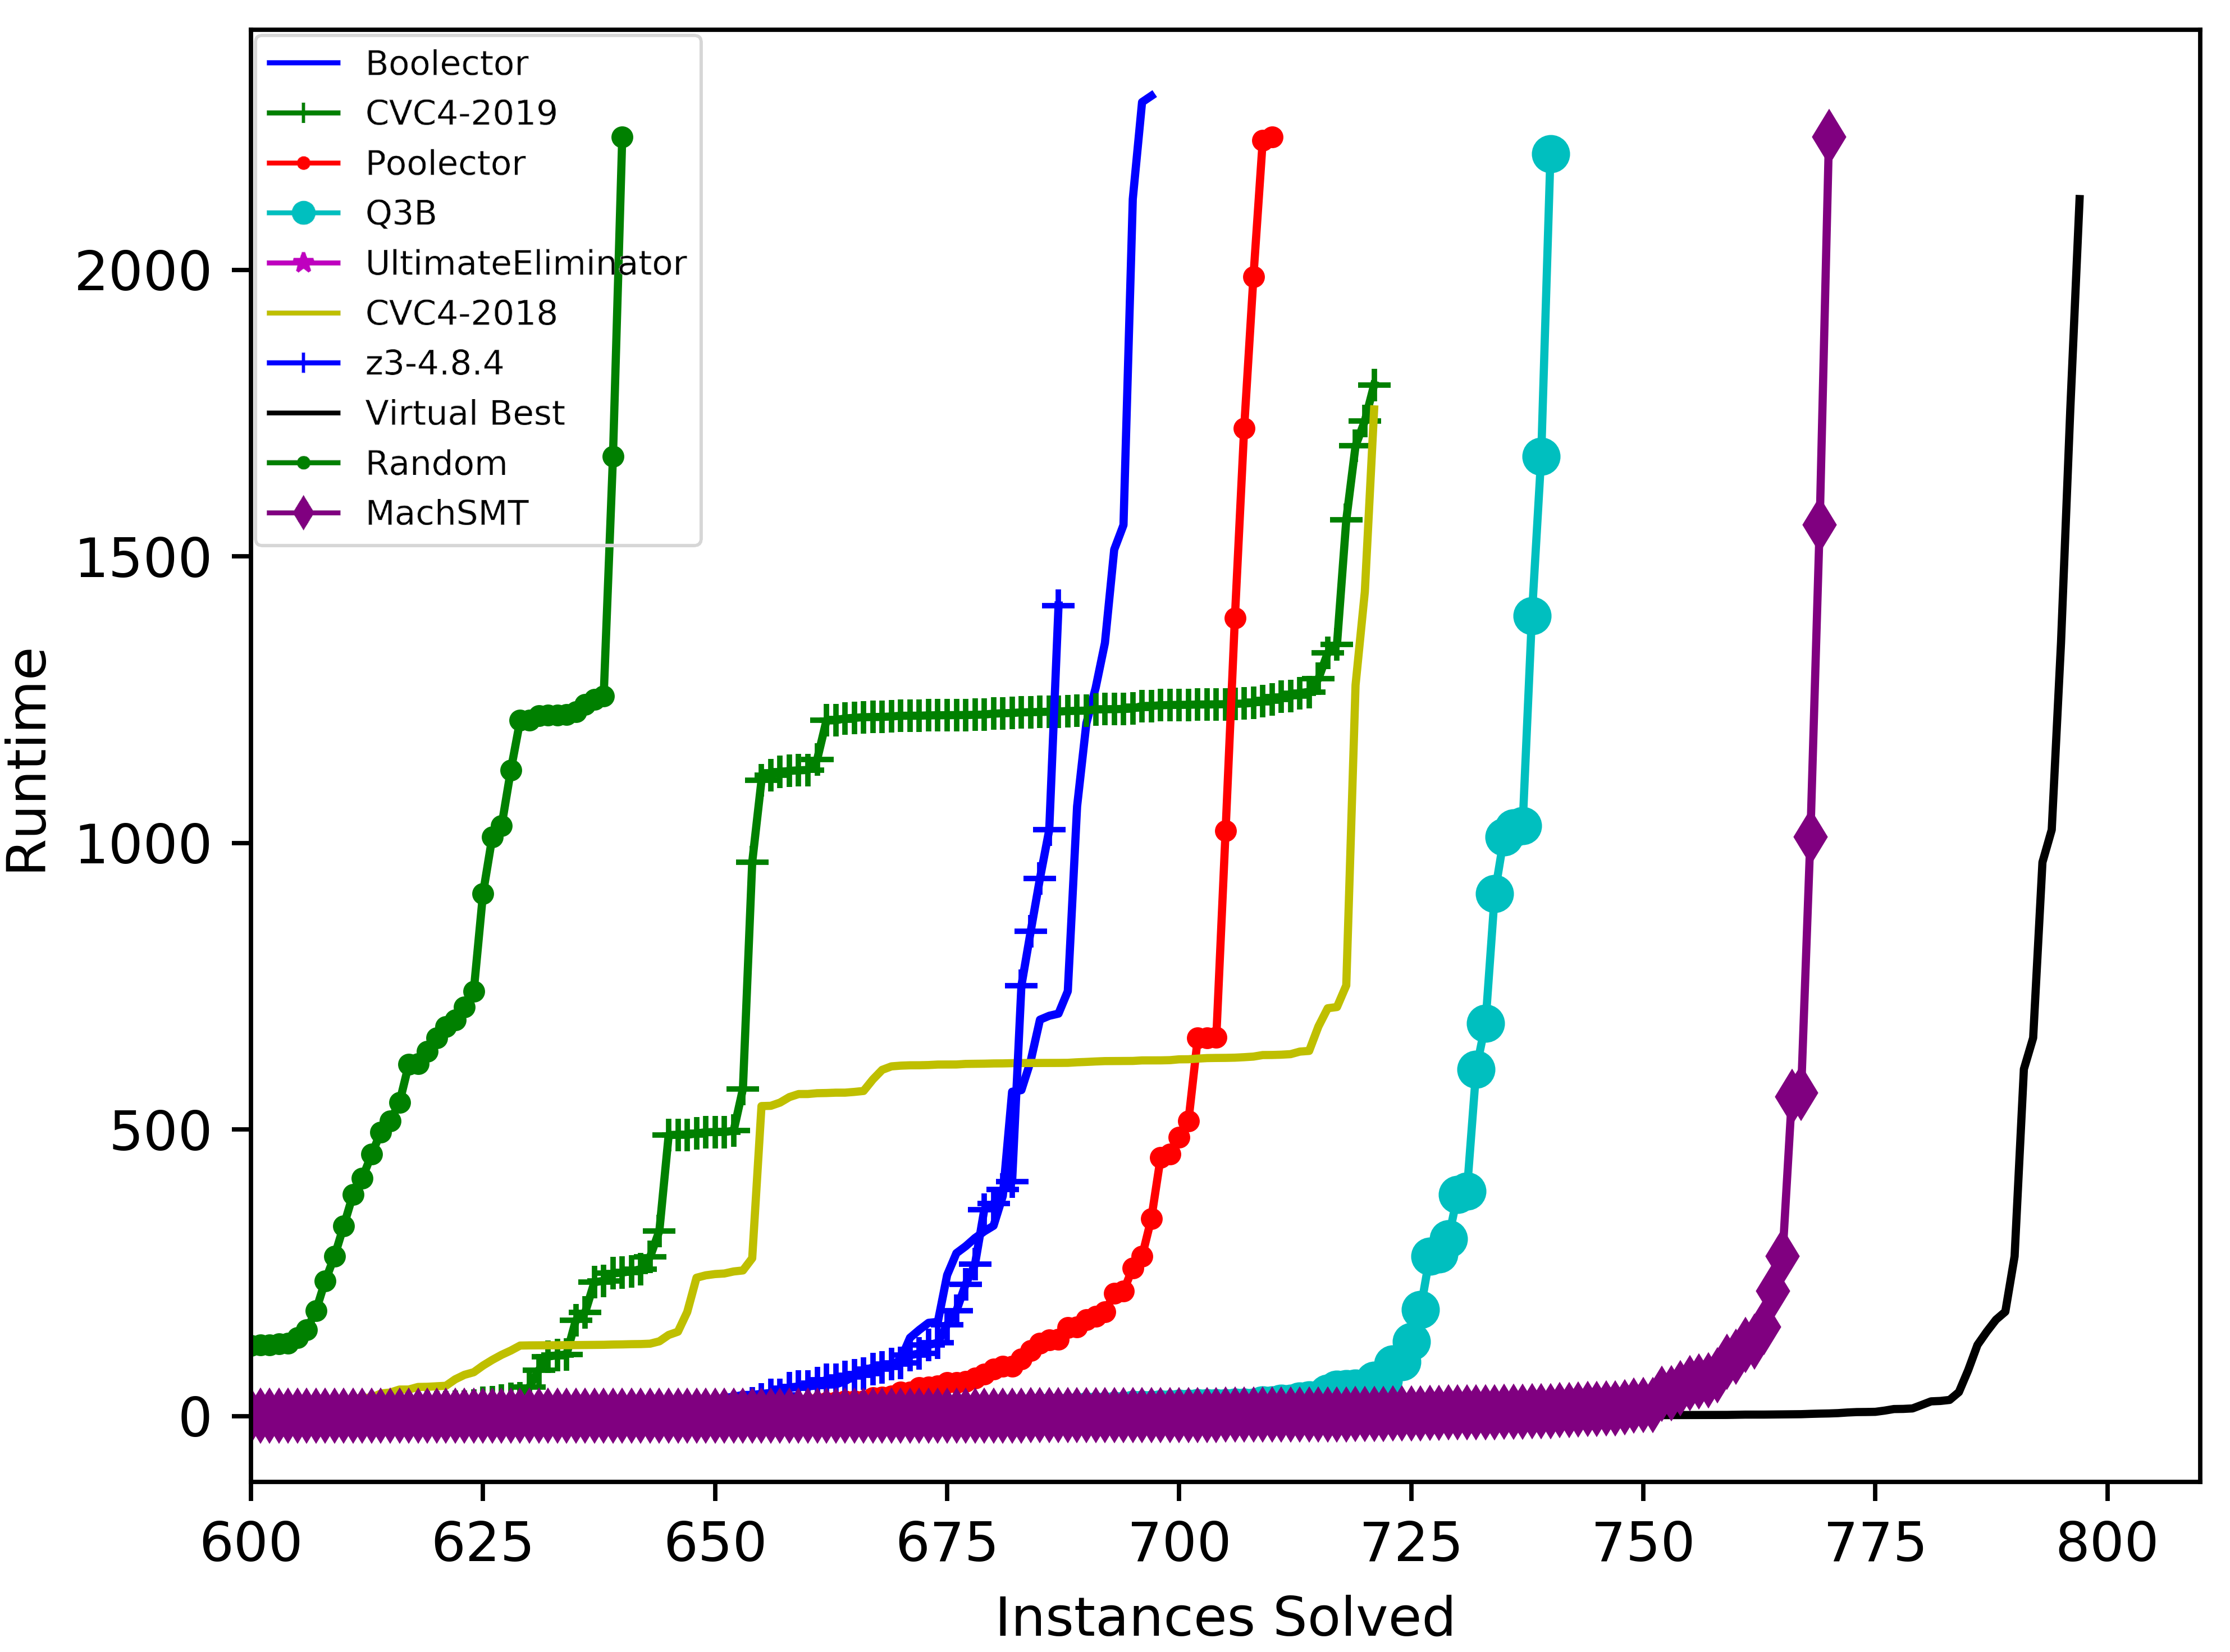
\includegraphics[width=\textwidth]{plot/machsmt_bv.png}
    \caption{BV (SQ)}
    \label{fig:machsmt_bv}
  \end{subfigure}
  \hspace{0.75em}
  \begin{subfigure}{0.48\textwidth}
    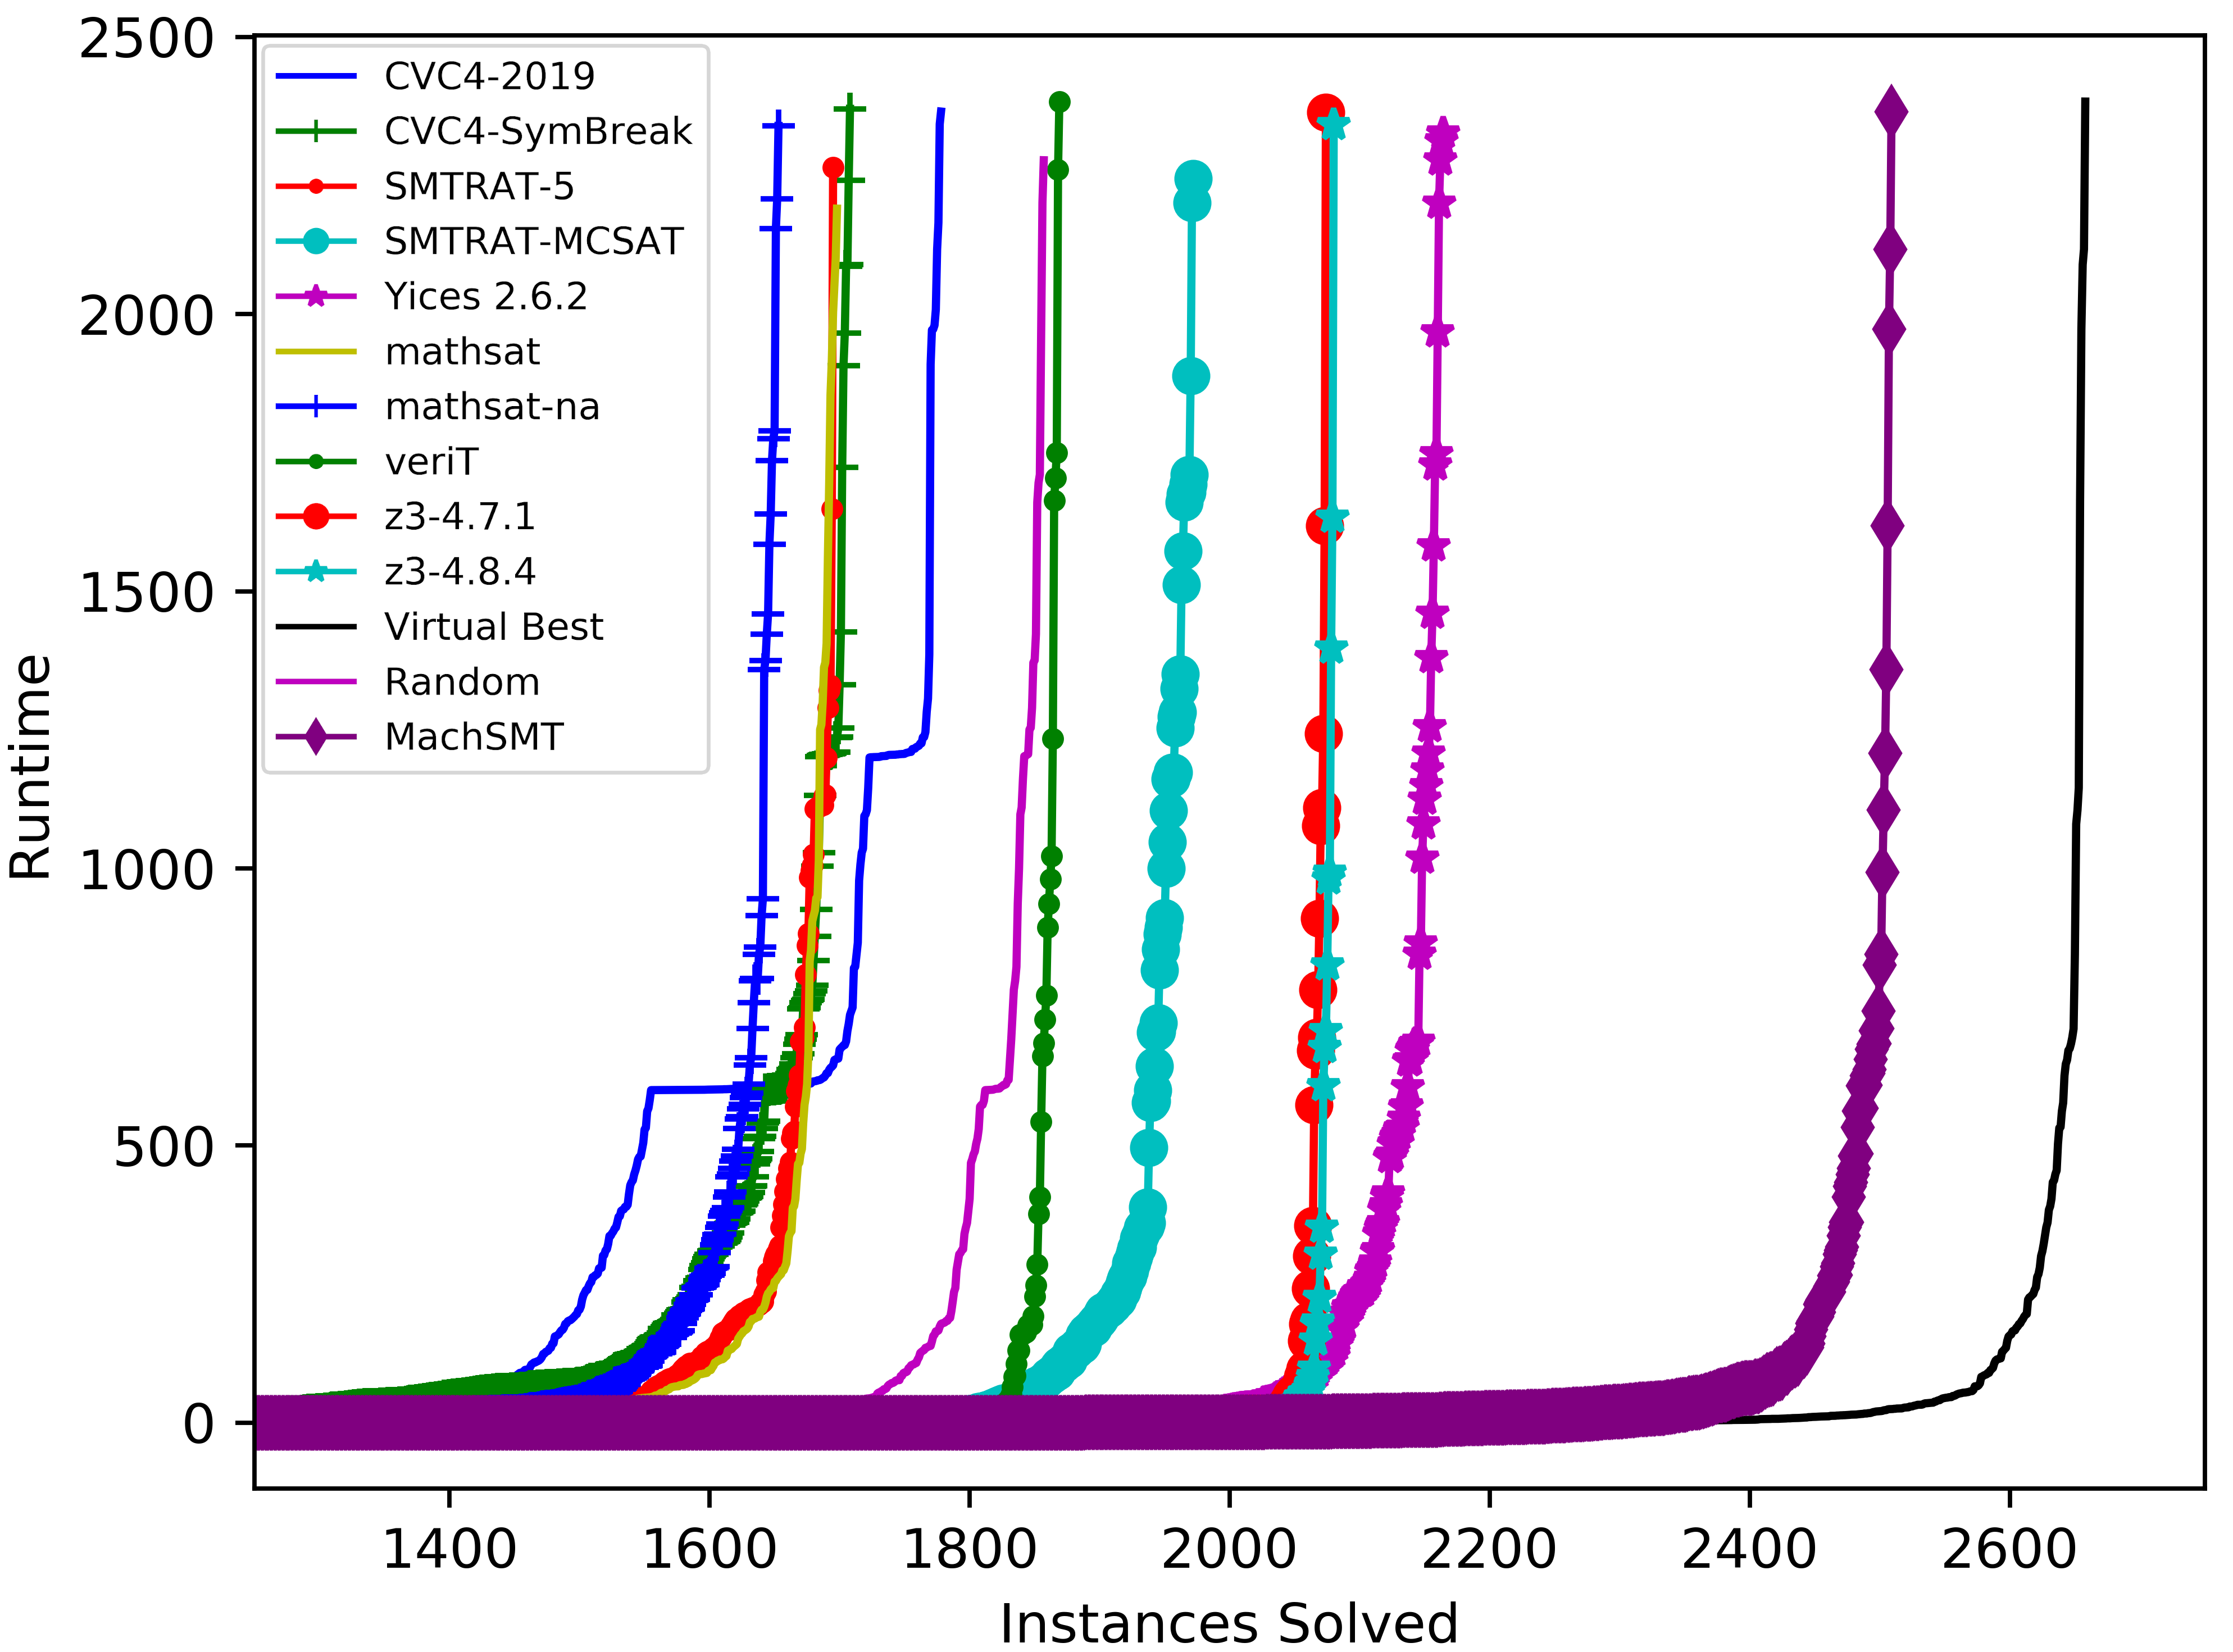
\includegraphics[width=\textwidth]{plot/machsmt_qf_nra.png}
    \caption{QF\_NRA (SQ)}
    \label{fig:machsmt_qfnra}
  \end{subfigure}\\[1.5em]
  \begin{subfigure}{0.48\textwidth}
    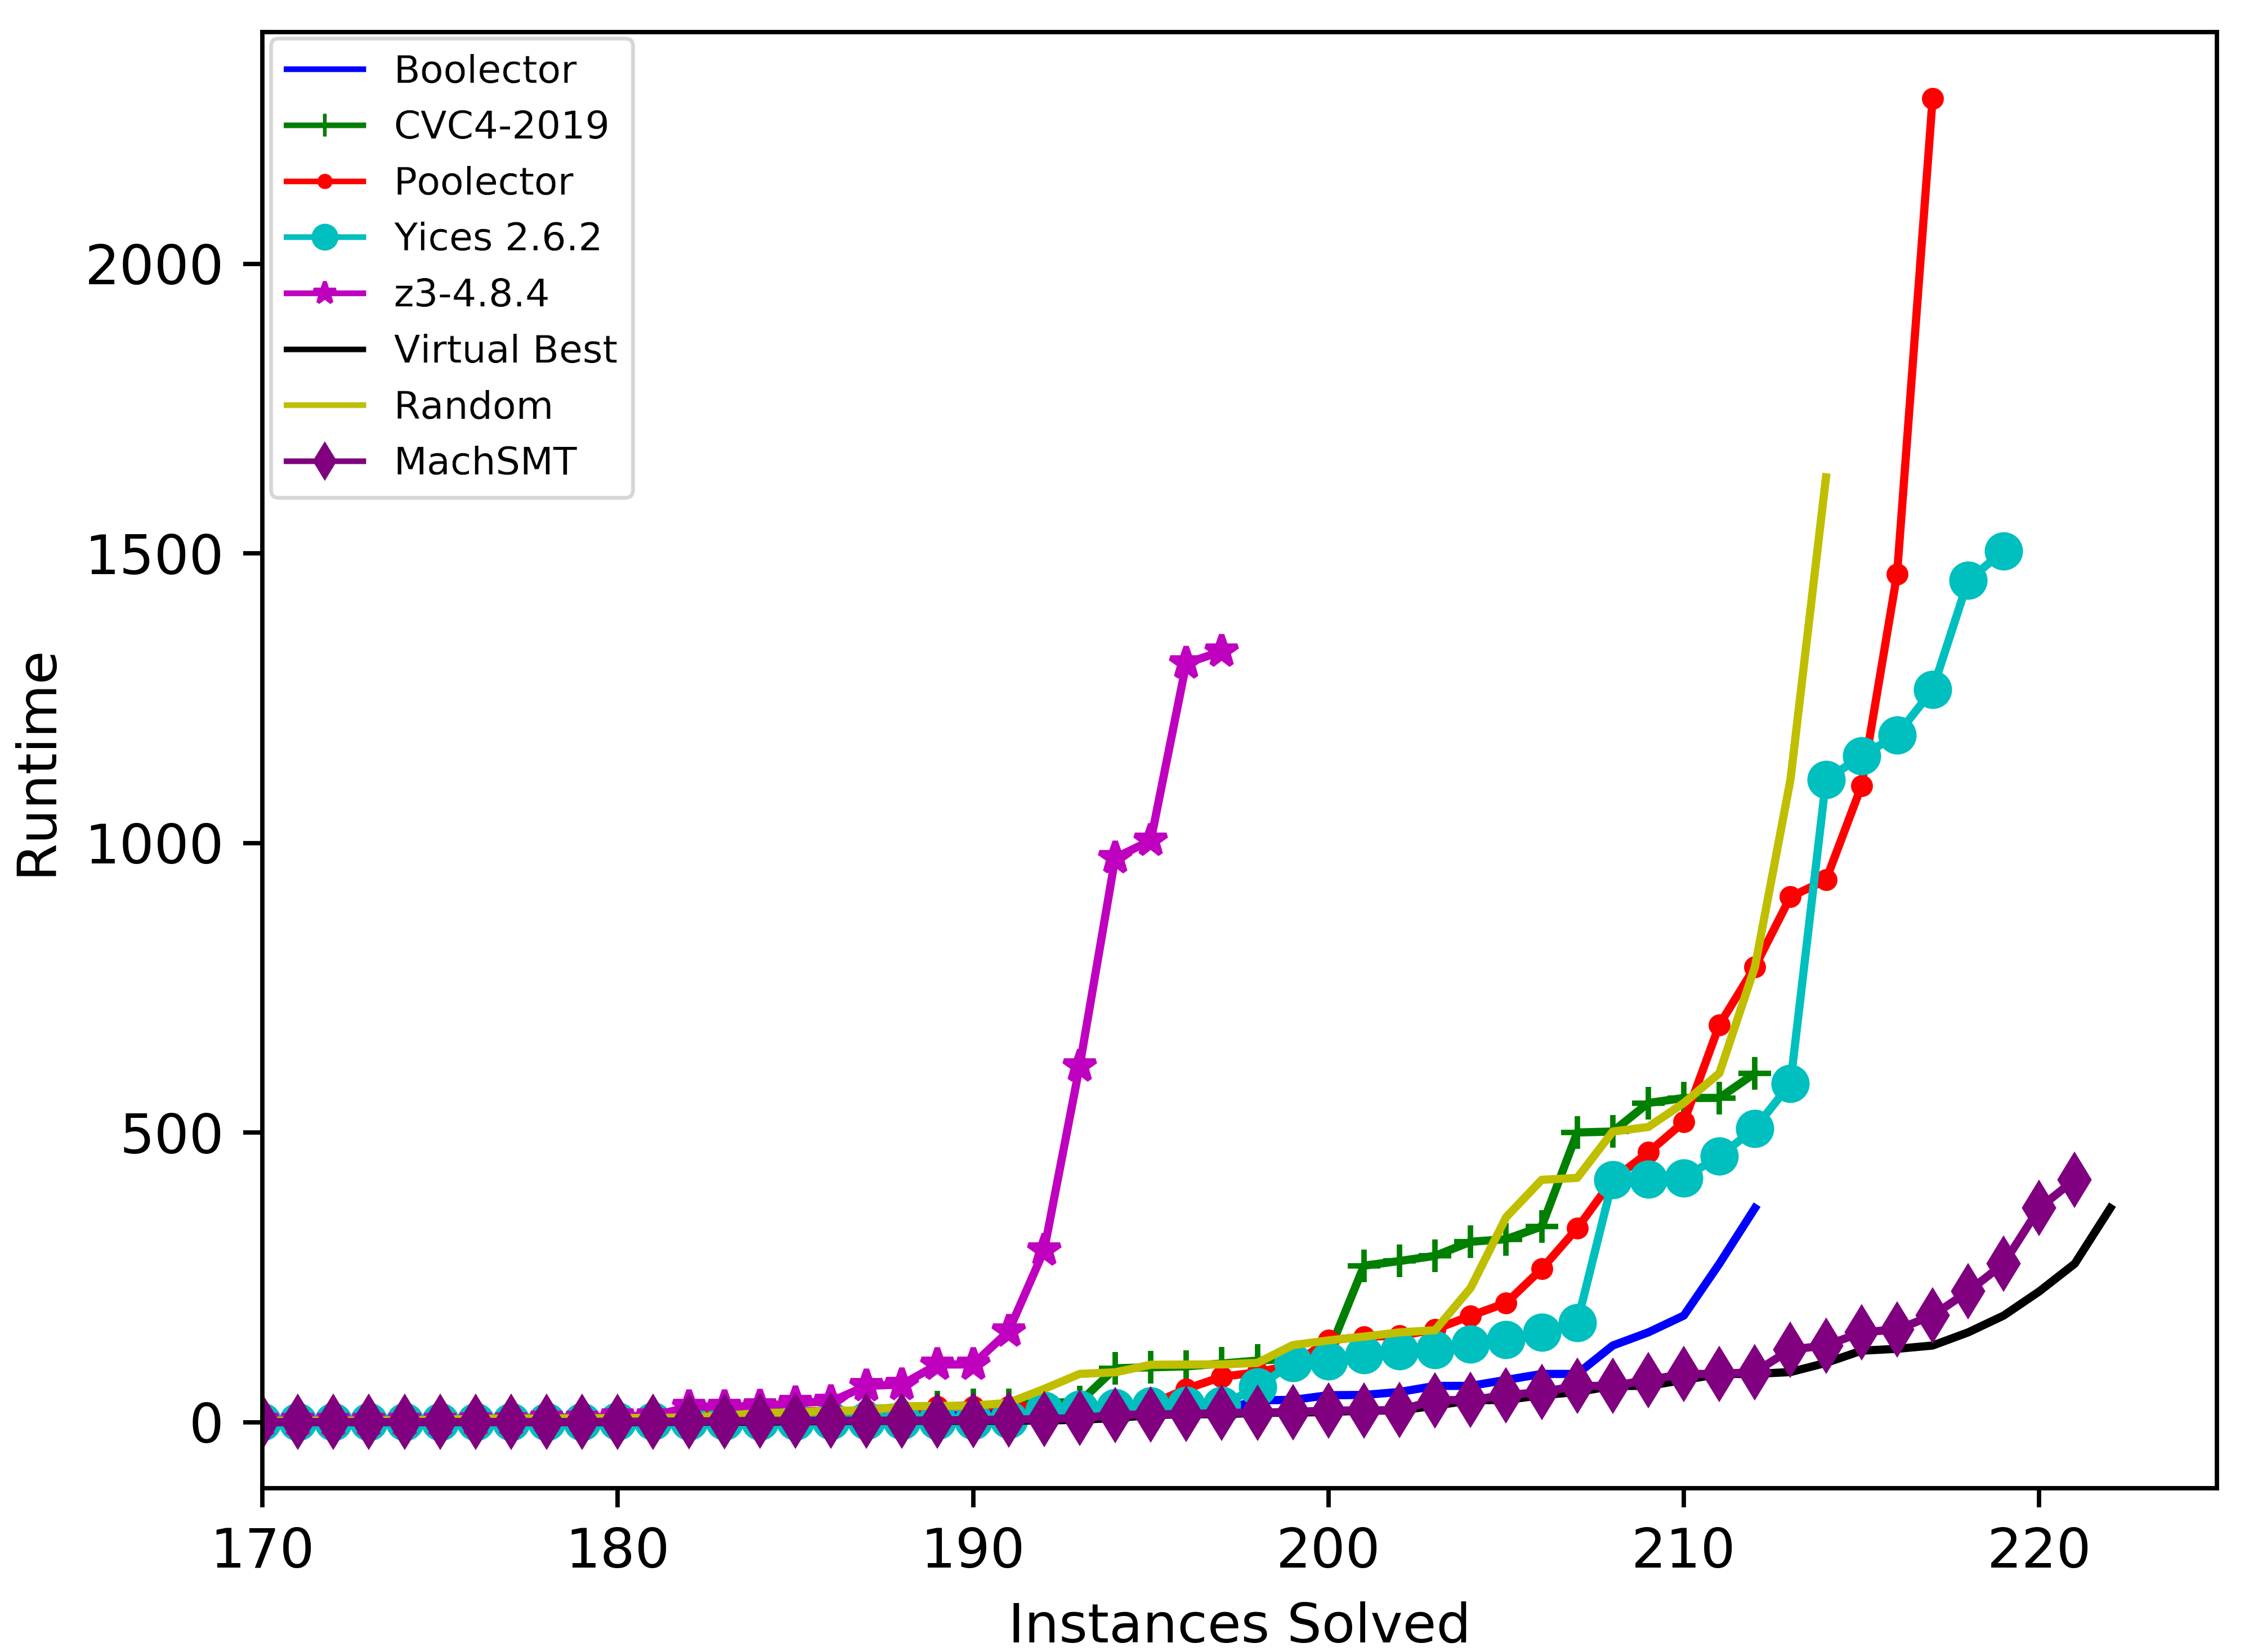
\includegraphics[width=\textwidth]{plot/machsmt_qf_ufbv.png}
    \caption{QF\_UFBV (SQ)}
    \label{fig:machsmt_qfufbv}
  \end{subfigure}
  \hspace{0.75em}
  \begin{subfigure}{0.48\textwidth}
    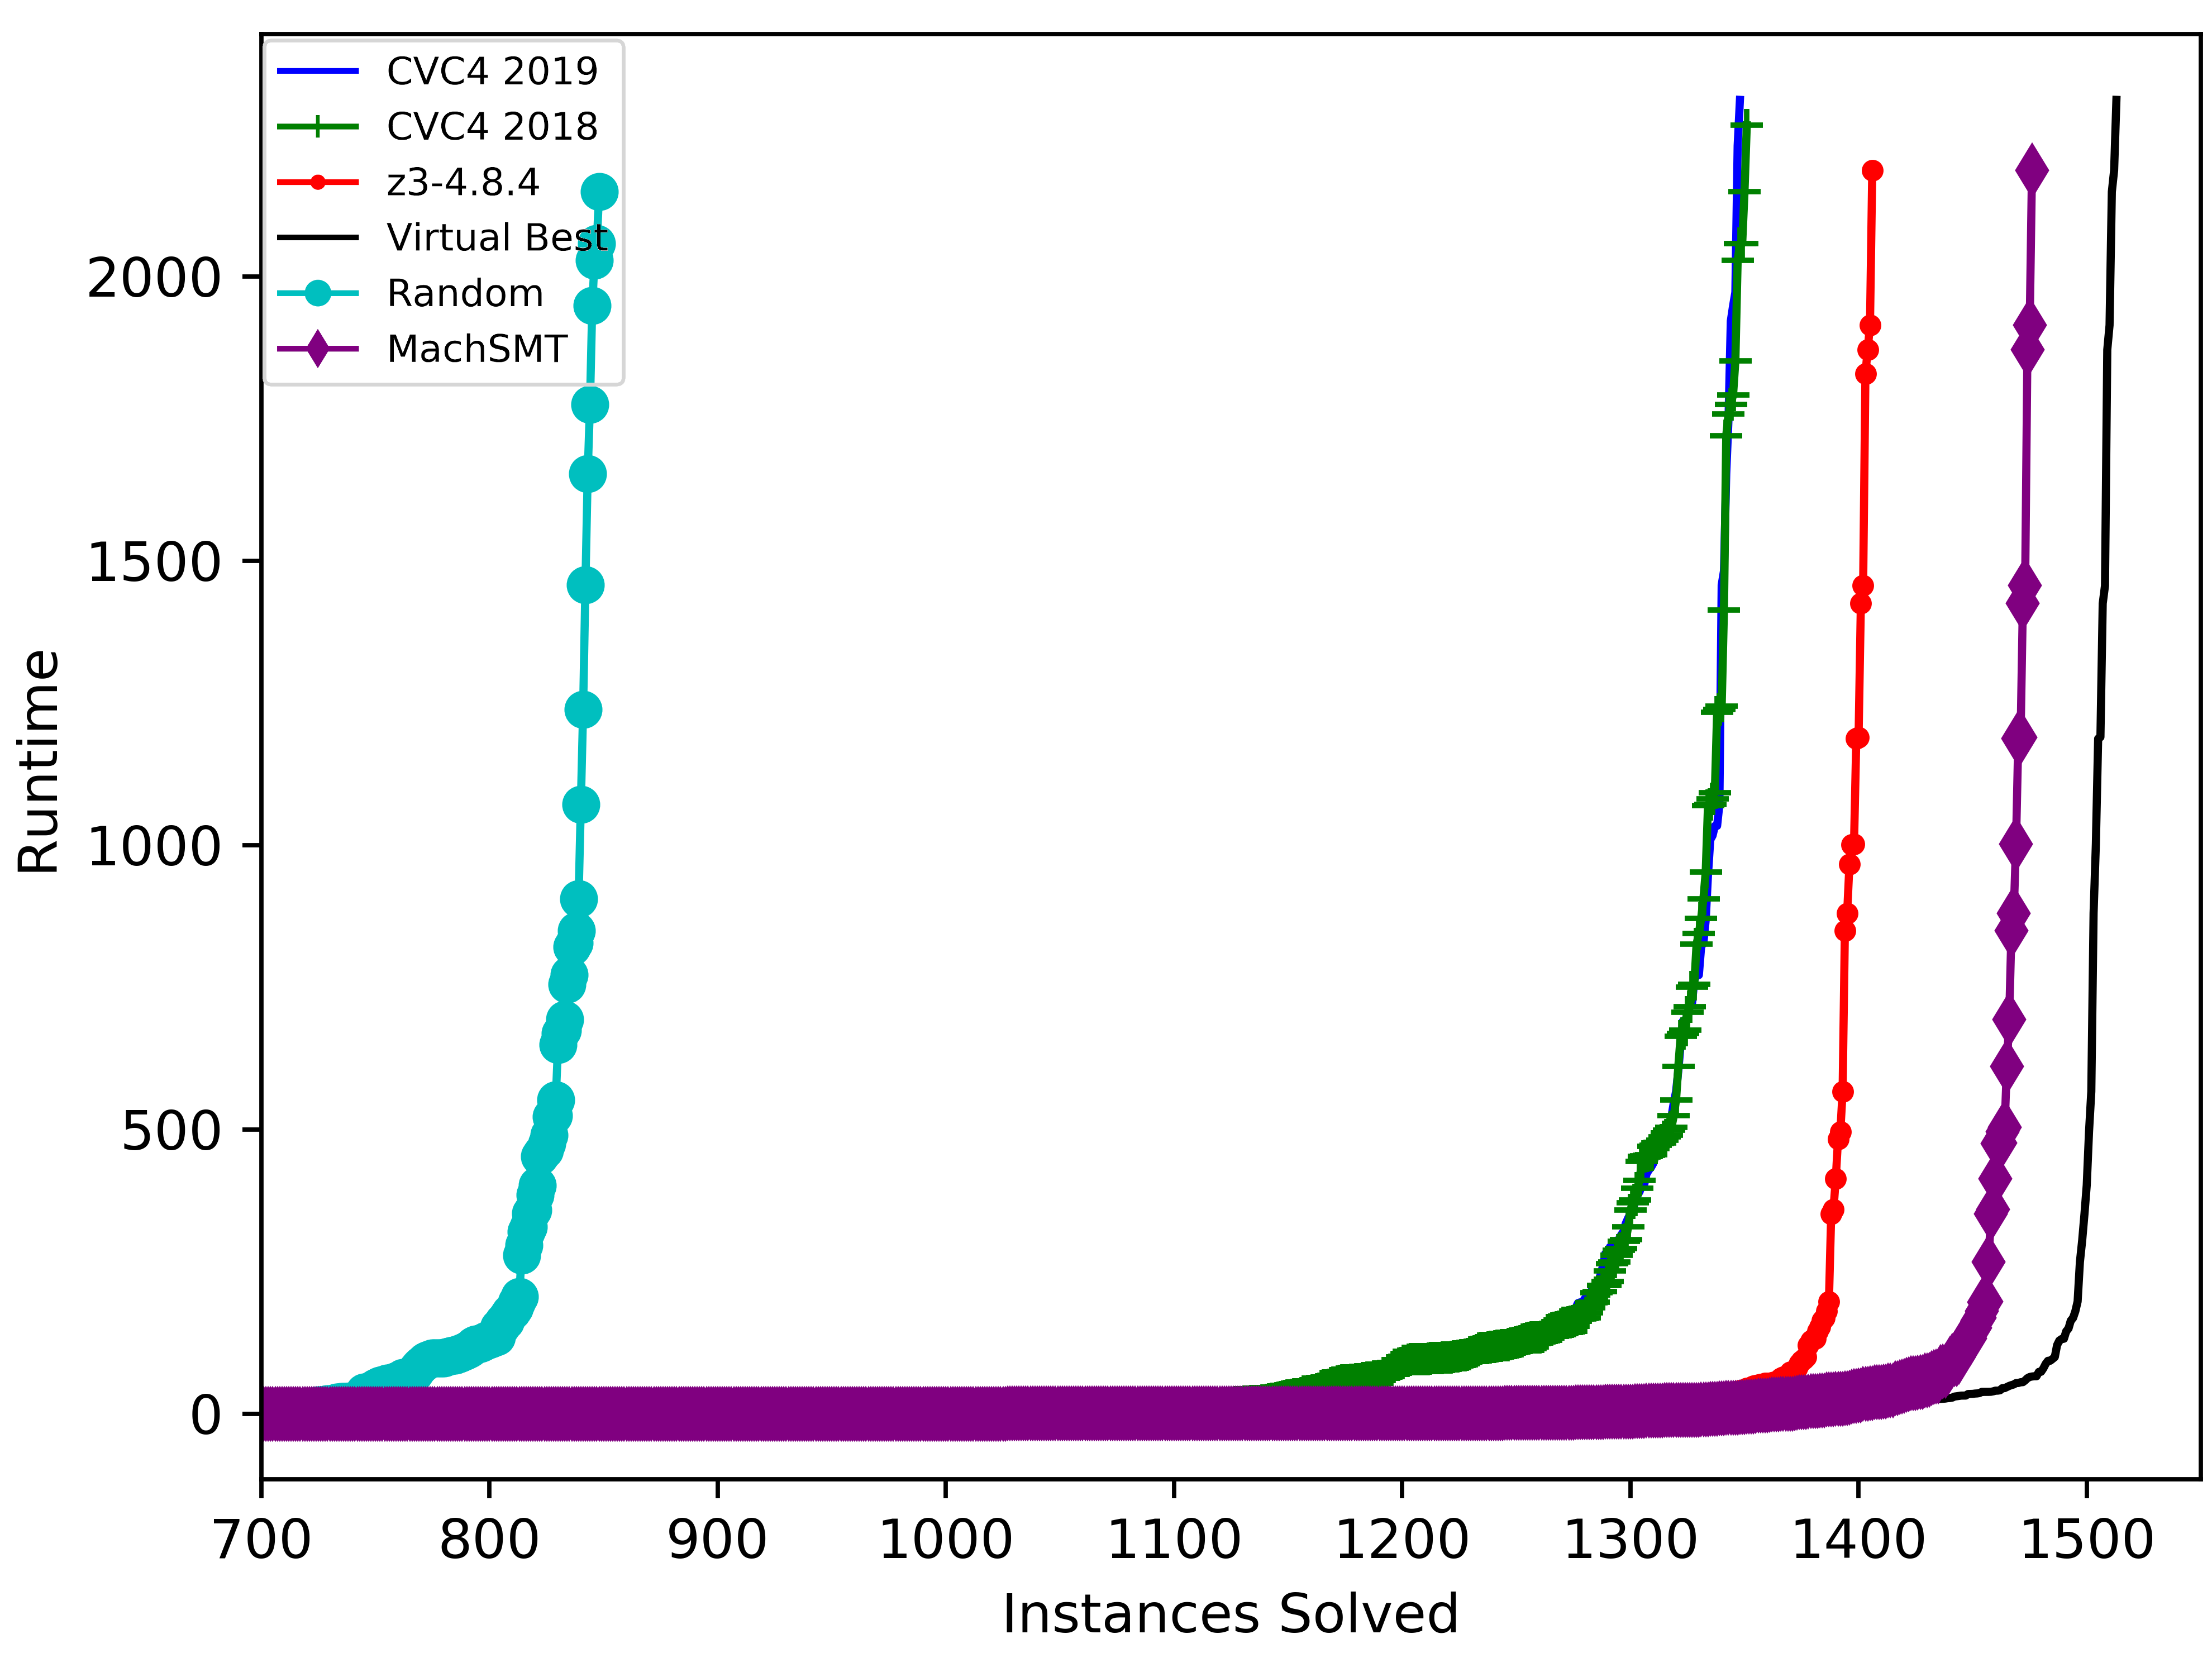
\includegraphics[width=\textwidth]{plot/machsmt_ufnia.png}
    \caption{UFNIA (UC)}
    \label{fig:machsmt_ufnia}
  \end{subfigure}

  \caption{MachSMT evaluated on selected SMT-COMP 2019 single query (SQ) and
           unsat core (UC) divisions. Random corresponds to MachSMT making
           random predictions without considering any EHMs.}
  \label{fig:machsmt_results}
\end{figure}



\bibliography{mybib}{}
\bibliographystyle{plain}
\end{document}
